\section{Trap Geometry}
Now that we have a better understanding of the types of ions used in trapped ion quantum computing, as well as some of the advantages and disadvantages they each have, we can turn our attention to the trapping configurations. 

When considering the possible geometries that an ion trap can have, we're essentially given two choices: one-dimensional (1D), also known as linear arrays; or two-dimensional (2D), sometimes called planar arrays, which is the basis for the 2D Coulomb crystals we're building up to. 

\subsection{Linear Arrays}
It may come as no surprise that the first quantum computers to be described using trapped ions made use of linear traps. Despite the simplistic geometry, all the necessary features of a quantum computer can be realized with linear ion traps. It's even possible to implement quantum gates between any set of ions in this scheme, not necessarily neighboring ions, for gates involving pairs, triplets, or any arbitrary number of ions. However, in practice, increasing the number of effective qubits is not an arbitrary task. Decoherence due to the environment interacting with the quantum system remains a significant challenge \cite{Cirac}.

Nevertheless, advances have been made that show how quantum computers based on linear arrays could provide solutions to difficult problems in materials design and molecular modeling through quantum simulation. In one example from 2017, Zhang \textit{et al.} successfully performed a quantum simulation of a dynamical phase transition (DPT) using up to 53 qubits in a linear ion trap. In this system, the qubits are coupled at long-range through their collective quantized motion due to Coulomb interactions. Each individual qubit is measured by a global long-range Ising interaction which has an efficiency of almost 99\%. This high efficiency makes it possible to measure many-body correlations between qubits in one shot, thereby allowing the DPT to be probed directly \cite{Zhang}.

The method employed by Zhang \textit{et al.} for confinement of long ion chains relied on a three-layer linear Paul trap with \ion{171}{Yb}{+} ions. Across the chain, ion spacing is anisotropic, ranging from \SI{1.5}{\micro\meter} at the center to \SI{3.5}{\micro\meter} towards the ends. As one might expect, the average lifetime of the chain scales inversely with the number of ions. At the maximum, 53 ions, an average lifetime of about 5 minutes was observed (which was sufficient for this experiment). The greatest factor in limiting the effective liftetime of the ion chain was Langevin collisions with residual background gas. When looking to scale up a system of this type, it will be crucial to implement cryogenic trap systems to reduce the pressure and collision energies \cite{Zhang}. 

More recently, a flexible scheme for maintaining efficient entanglement between ions in a long chain as the size scales up has been introduced by Leung and Brown. By utilizing both amplitude and frequency modulation, they show it's theoretically possible to apply high-fidelity pulse sequences to drive transverse motional modes, which can suppress gate errors (See Fig. \ref{fig:Linear Trap}). Those pulses in turn require greater power to operate, so there is a trade-off between higher tolerance against errors and power efficiency.

\begin{figure}[h]
    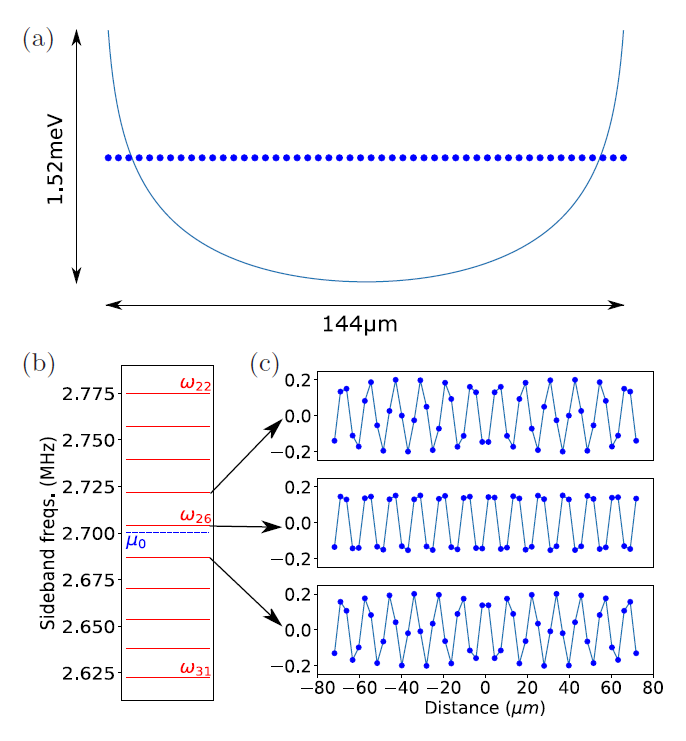
\includegraphics[width=\linewidth]{Leung - Linear Trap.png}
    \caption{(\textbf{a}) An idealized distribution of ions in a trap with $r=0.95$. The minimum trap depth required to trap all 50 ions is \SI{1.52}{\milli\electronvolt}. (\textbf{b}) The middle band of the transverse motional frequencies. The approximate driving frequency is represented by the dashed blue line where $\mu_0 = \omega_{26} - \SI{3.7}{\kilo\hertz}$. (\textbf{c}) The normalized 25th to 27th transverse motional modes. In the center is the 26th mode which exhibits a valuable unformity making it an excellent candidate for two-qubit entanglement. From \textit{Entangling an arbitrary pair of qubits in a long ion crystal} \cite{Leung}.}
    \label{fig:Linear Trap}
\end{figure}

While linear arrays remain a promising area of research, there are some shortcomings to this particular trap geometry. In general, as the size of the ion chain increases, there is weaker motional coupling between ions with ion-ion coupling strength falling off as $1/s^\alpha$ where $s$ is the distance between two ions. That then leads to limitations such as decreasing speed of qubit gates and a corresponding increase in noise-induced heating in the system (due to the gates taking longer) \cite{Bruzewicz}.

Those challenges could be overcome if the ion chain were to be broken into smaller pieces, or modules, which could perform operations at high-speed and efficacy within an individual module. That type of scheme would require some way of moving the quantum information between modules or even moving the ions themselves. This is possible given variable voltages in the ion trap electrodes that control the trapping potential. We can imagine breaking off subsets of ions from their modules and combining them in a new module to allow interaction. Then by returning them to their original positions, that quantum information has become more widely distributed. However, this process of splitting and joining many ion chains comes with it's own challenges and the ability to do it quickly and with high fidelity will be constrained by the size of the ion chain \cite{Bruzewicz}.

While distribution of quantum information is not impossible in a 1D linear array (and quantum computing is certainly possible), there are improvements that can be made in some areas by expanding to a 2-dimensional array (See Fig. \ref{fig:Trap geometries}).

\subsection{Planar Arrays}
When looking to scale up trapped-ion systems, 2D architectures have been proposed to mitigate the problems faced by larger linear arrays. In a linear chain, the ions are only weakly confined along the axial direction of the chain. Because of this, high heating rates can occur due to the axial motional modes making laser cooling a challenge. It also becomes a issue for laser-addressing the outer ions as the length of an ion chain grows. Just keeping a long one-dimensional chain in a linear form requires extremely anisotropic traps that ultimately limits how many ions can be controlled without introducing errors. Introducing a second spatial dimension can be shown to overcome these obstacles related to heating, quantum state manipulation, and more \cite{Kiesenhofer}.

Having access to additional spatial dimensions also allows for the ability to simulate complex many-body systems. For example, the study of frustrated magnetic materials (where the natural tendency of magnetic moments to align with each other is hindered or frustrated by the geometric arrangement of atoms in the crystal lattice) becomes an intractable problem for classical computers when the number of spins becomes very large. A trapped-ion quantum simulator could be used to simulate lattice spin systems and even allow us to investigate the nonequilibrium quantum dynamics of the system \cite{Yoshimura}. 

Two-dimensional or planar arrays are built on much of the same concepts as the linear arrays we just discussed. There are various trapped-ion architectures that utilize 2D arrays including microtrap arrays, Penning traps, and multizone trap arrays. In general, Penning traps and microtraps have large ion separation which makes them ineffective for fast quantum gates that rely on the distance dependent ion-qubit interaction.
\begin{figure*}[t]
    \centering
    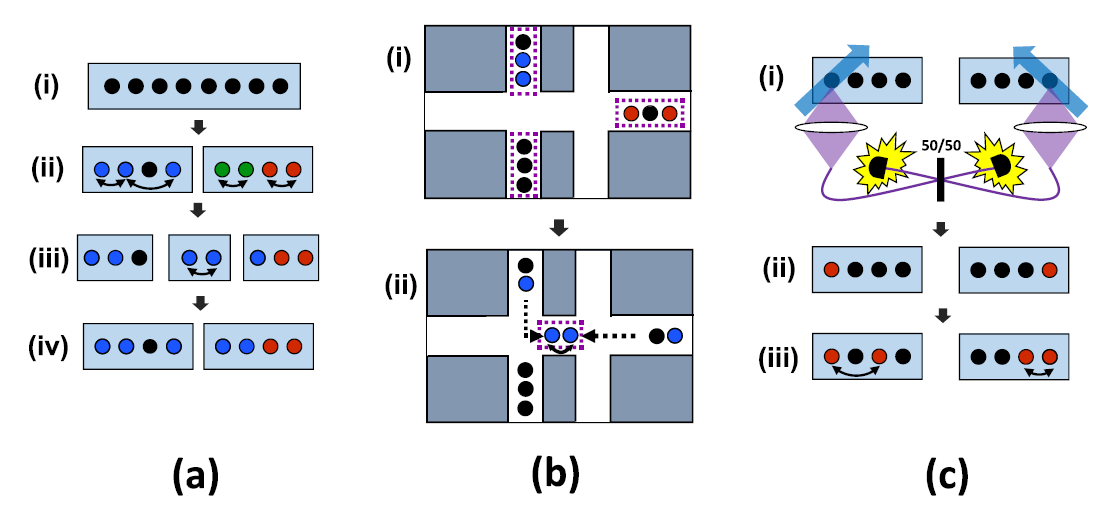
\includegraphics[width=\textwidth]{Bruzewicz - Architectures.png}
    \caption{Illustration of how entanglement can be achieved in various trapped-ion architectures. Black dots indicate no entanglement while like colors indicate entanglement between those ions. (\textbf{a}) Linear ion chain. (i) The qubits are initially in one long chain and no entanglment has ocurred. (ii) The chain is split into modules (blue boxes) where high-fidelity entangling gates can be performed. (iii) Ions from different modules are then combined in a new module where another entangling gate can be performed. (iv) The qubits are then returned to their original positions. (\textbf{b}) 2D array. (i) Qubits are separated into modules on a 2D array; they may or may not be entangled. They are kept in "memory zones" (dotted boxes) which are optimized for long coherence times. (ii) To entangle qubits from different modules, the ions are shuttled into an "interaction region" (dotted box) where entangling gates are performed. They are then shuttled back to their previous modules and the process can be repeated as needed. (\textbf{c}) Photonic interconnects. This example is of a linear array, but the concept can be applied to 2D arrays. (i) Each module contains a dedicated communication ion which is excited by a laser (blue arrows). The excited ions emit photons (purple) that are entangled with the internal ion state. The photons are directed through optics (ovals) into a 50/50 beam splitter where they interfere. (ii) If photons are simultaneously detected at the single-photon detectors (black hemispheres), that indicates the communication ions have been entangled. (iii) Intra-module entangling gates can then be performed to distribute the entanglement. From \textit{Trapped-ion quantum computing: Progress and challenges} \cite{Bruzewicz}.}
    \label{fig:Trap geometries}
\end{figure*}
 Penning traps also require fast rotation of the ion crystal which significantly increases the difficulty of individually addressing qubits \cite{STWang}.

For those reasons, Paul traps are preferred in many quantum computer applications. Paul traps can operate with lower magnetic fields, stationary 2D crystals, and facilitate individual addressing by laser beams. The main challenge in using Paul traps for producing 2D ion crystals comes from micromotion due to the oscillating applied electric field \cite{YeWang}. This type of driven motion is present in all radio-frequency (RF) ion traps, including 1D linear traps. However, micromotion can be minimized in the 1D case by placing the ions along the line corresponding to zero electric field amplitude. For 2D or even 3D cyrstals, the problem becomes more difficult and requires more sophisticated methods to mitigate the micromotion \cite{Kato2}.

We can't say that 2D arrays are necessarily better than their 1D counterparts, but they do seem to be a promising path forward for scalable quantum technology. In the remainder of the paper, we'll take a closer look various platforms that utilize two-dimensional Coulomb crystals and how researchers are dealing with the challenges inherent in this architecture.